\section{Evaluation}
\label{sec:experi}

\subsection{Setup and protocol}
\label{sec:setup}
All GPU systems run on one NVIDIA RTX 5090: 170 SMs, and a $101{,}376$-byte
opt-in shared-memory limit per block, which is the budget the resident table
competes for. The six datasets span 768 to 3{,}072 dimensions and 1.0M to
17.8M vectors; Figure~\ref{fig:frontier} labels each with its shape.

We report Recall@10 against true top-10 ground truth; because $c_k$ scales with
$\alpha k$, other $k$ are not established. Timing runs host query input to host
result output, and frontiers use steady-state throughput at batch 1{,}024,
which Section~\ref{sec:rq5} shows is a consequential choice; batches are not
enlarged by duplicating the roughly 1k available queries, since duplication
alone raises throughput (Table~\ref{tab:neg}). Nsight Compute counters were
unavailable in the container (\texttt{ERR\_NVGPUCTRPERM}), so every occupancy
statement is an analytical resource-budget calculation. Recall differences
below $10^{-3}$ across builds, and below $10^{-4}$ within one index, are noise;
the CPU comparison buckets at $10^{-3}$ accordingly.

Baselines are the cuVS implementations of IVF-RaBitQ~\cite{ivfrabitq}, IVF-PQ
and CAGRA~\cite{cagra} in fp32 and int8. The frontier's comparison line is the
IVF-routed family, which shares JHQ's routing structure, build cost and
interface; CAGRA is a graph index and is reported separately. The CPU baseline
is the authors' own artifact on the same host, threads pinned, sweeping
$(\alpha,\mathit{nprobe})$ as the GPU side does.

\subsection{RQ1: where does JHQ actually lead?}
\label{sec:rq1}
Figure~\ref{fig:frontier} gives the measured frontiers and Table~\ref{tab:front}
reduces them to one question: at each matched recall, which system is fastest?
Among IVF-routed methods JHQ owns 17 of the 24 comparable cells and IVF-RaBitQ
the other 7, by $1.1$--$1.4\times$. Two choices make that the baseline's own
best case. IVF-RaBitQ is run at whichever of cuVS's four search kernels is
fastest on each dataset, swept rather than fixed: the single kernel our earlier
runs used is not the best on three of the four, and costs it $5$ to $11\%$
there. And its coarse quantiser is trained at the cuVS default of 256 points a
centroid against JHQ's 39 --- $5.8$ to $6.6\times$ the budget --- worth up to
$0.039$ recall to it at shallow probe depths. We leave both in its favour and
report the build-time consequence below.

\begin{table}[tbp]
  \centering
  \caption{Fastest system at each matched recall, batch 1{,}024, with its margin
  over JHQ. \textsf{int8} and \textsf{fp32} are cuVS CAGRA, \textsf{RaBitQ} is
  cuVS IVF-RaBitQ; ``--'' is a recall no two systems both reach. JHQ is fastest
  in 17 of 24 cells; the graph baseline is reported in the text.}
  \label{tab:front}
  %% generated by figures/table_frontier.py -- do not edit
\begin{tabular}{lrrrrrr}
\toprule
& \multicolumn{6}{c}{fastest system at Recall@10}\\
\cmidrule(l){2-7}
dataset & $0.90$ & $0.93$ & $0.95$ & $0.97$ & $0.98$ & $0.99$ \\
\midrule
vogue-768 & C-int8 $2.7\times$ & C-int8 $2.0\times$ & C-fp32 $1.1\times$ & RaBitQ $1.0\times$ & RaBitQ $1.1\times$ & \textbf{JHQ} \\
arxiv-768 & C-int8 $2.9\times$ & C-int8 $2.9\times$ & C-int8 $2.5\times$ & C-fp32 $1.4\times$ & C-fp32 $1.4\times$ & RaBitQ \\
bge-m3 & C-int8 $2.4\times$ & C-int8 $1.7\times$ & -- & -- & -- & -- \\
stella-trec24 & -- & -- & -- & C-int8 $2.6\times$ & -- & -- \\
openai3-1536 & C-int8 $1.9\times$ & C-int8 $1.6\times$ & C-int8 $1.3\times$ & \textbf{JHQ} & \textbf{JHQ} & -- \\
openai3-3072 & C-int8 $2.4\times$ & C-int8 $2.1\times$ & C-int8 $1.6\times$ & \textbf{JHQ} & RaBitQ $1.1\times$ & RaBitQ $1.4\times$ \\
\bottomrule
\end{tabular}

\end{table}

On bge-m3 and stella-trec24 the tested cuVS IVF-RaBitQ build path runs out of
memory and CAGRA fp32 does not fit the card, and on stella-trec24 IVF-PQ fails
too; JHQ indexes all six. These are the tested library's paths on this device,
not a property of the algorithms. One row is excluded throughout:
stella-trec24's CAGRA-int8 point at Recall@10 $0.9692$ is
\texttt{status=CONTAMINATED} in the harness's own record.

\begin{figure}[tbp]
  \centering
  
\includegraphics[width=\linewidth]{figs/fig_frontier.pdf}
  \caption{Measured Recall@10--QPS frontiers, batch 1{,}024. Four datasets carry
  complete JHQ/IVF-RaBitQ curves; the two largest show the baselines that could
  be built and searched on the tested card. Sweep endpoints are measured
  endpoints, not architectural recall ceilings.}
  \label{fig:frontier}
\end{figure}

CAGRA is faster than JHQ where both run and the recall target is not high:
CAGRA-int8 leads in 13 of the 15 cells they share by $1.3$--$2.9\times$, and
below Recall@$10{=}0.95$ in 10 of them by $1.6$--$2.9\times$; CAGRA-fp32 leads
in 8 of 21 by $1.1$--$1.5\times$. What it costs is build time.
Figure~\ref{fig:build} gives both variants beside JHQ: where CAGRA int8 is the
faster searcher, its throughput repays the build gap only after $1.6$M to
$8.9$M queries. Neither CAGRA variant builds on stella-trec24 within the card,
and fp32 does not build on bge-m3 either.

\begin{figure}[tbp]
  \centering
  
\includegraphics[width=\linewidth]{figs/fig_build.pdf}
  \caption{Index build time, log scale. Bars are the median over swept
  configurations and repeat builds and whiskers their range, not a confidence
  interval. JHQ's bar is one cold training plus its median encode: training is
  cached after a dataset's first row and encoding is not. Each baseline's
  fastest build per dataset is used.
  The coarse-training budgets differ and are not controlled here: JHQ trains at
  39 points a centroid, cuVS defaults to 256, so IVF-RaBitQ trains on $5.8$ to
  $6.6\times$ as many points. Part of its build gap is that budget rather than
  the index, and the same budget buys it better centroids at search time.}
  \label{fig:build}
\end{figure}

\subsection{RQ2: does the design prediction hold?}
\label{sec:rq3}
Section~\ref{sec:designspace} predicted that reducing table state helps only
until extra lookups outweigh the residency saved. Figure~\ref{fig:lutgroups}
varies $G$ with the represented distance fixed. If state alone governed
throughput, $G{=}4$ and $G{=}8$ should win, since they store fewer entries than
$G{=}2$. They do not: $G{=}2$ wins all eight configurations in
Figure~\ref{fig:lutgroups}(a), and throughput falls monotonically as lookups
per candidate rise. Its narrowest win is not resolvable --- a second phase of
the same run puts that cell on the other side of zero --- which is why the
design is stated as a regime rather than a rule.

The sharpest form of the argument is internal to the losers. $G\cdot 2^{8/G}$ is
$16$ for both $G{=}4$ and $G{=}8$, so the pair holds the table footprint fixed
and differs only in the lookups and address arithmetic it needs. Residency is
constant, issued work rises, and throughput falls with it --- by $5.8$ to
$38.3\%$, widening with probe depth.

The regime change with $M$ appears as predicted: factorisation is worth a few
percent at $M{=}96$ and up to $+53.8\%$ at $M{=}384$. At $M{=}96$ the gain
neither rises reliably nor exceeds the noise, for the same reason as the
ambiguous cell above --- the full table misses the carveout by $2$\,KiB there
against $290$\,KiB at $M{=}384$, so there is almost no residency to win back.

\begin{figure}[tbp]
  \centering
  
\includegraphics[width=\linewidth]{figs/fig_lutgroups.pdf}
  \caption{(a) $G{=}2$ wins all eight configurations of the granularity sweep
  although $G{=}4$ and $G{=}8$ store fewer entries and occupy the same footprint
  as each other; every line is one probe depth, normalised to its own $G{=}2$.
  (b) Factorisation matters far more at $M{=}384$ than $M{=}96$ and stays
  largely complementary to packed loading. The two panels are different phases
  of the run --- (a) the granularity sweep at
  $\mathit{nprobe}\in\{8,32,128,512\}$, (b) the two-by-two table$\times$layout
  phase at $\mathit{nprobe}\in\{32,128,512\}$ --- and are counted separately.}
  \label{fig:lutgroups}
\end{figure}

\subsection{RQ3: can the byte-count explanation be rejected?}
\label{sec:rq4}
Table~\ref{tab:neg} collects the controls that vary bytes and issued work
independently; its third column names the version of ``fewer bytes is faster''
each row rejects. Removing almost all table state loses heavily while
\emph{raising} the resident-block count the shared-memory budget implies, so
neither residency nor attainable occupancy alone is the bottleneck. Moving
identical bytes in 32-bit words gains up to $66\%$, rising with probe depth for
the reason the factorisation gain does: a load is paid once per candidate per
subspace. And table construction is under $3\%$ of a batch, so faster table
building does not explain factorisation either.

\begin{table}[tbp]
  \centering
  \caption{Controls that separate bytes moved from work issued. Every row holds
  the represented distance fixed.}
  \label{tab:neg}
  \begin{tabular}{lll}
    \toprule
    change & effect on throughput & what it rules out \\
    \midrule
    table-free exact distance & $-30$ to $-52\%$ & least state is fastest \\
    $G{=}8$ against $G{=}4$   & $-5.8$ to $-38.3\%$ & same footprint, same speed \\
    packed 32-bit loads       & $+1$ to $+66\%$ & bytes moved predict speed \\
    private probe cursor      & $-1.4$ to $+148.5\%$ & loop work is negligible \\
    fused residual refinement & $-14.2\%$, $-14.8\%$ & fewer kernels is better \\
    query duplication $D{=}8$ & $+4$ to $+26\%$ & reuse alone drives the scan \\
    \bottomrule
  \end{tabular}
\end{table}

Static instruction counts complete the argument without a profiler.
\texttt{cuobjdump -sass} on \texttt{scan\_ivf\_coalesced\_kernel} finds exactly
$G$ generic loads and $G{+}1$ floating-point adds per unrolled subspace
iteration, giving $5.0$, $13.0$, $25.0$ and $50.4$ static instructions per
candidate--sub\-space at $G{=}1,2,4,8$. One statement then needs no model:
\emph{$G{=}1$ issues $5.0$ against $G{=}2$'s $13.0$, holds 256 table entries a
subspace against 32, and is slower at most operating points anyway}. Instruction
count predicts it should be fastest; the state it holds is the one thing that
separates them. Sizing that shortfall means extrapolating a fit beyond its
range, so we read its sign and trend only.

\subsection{RQ4: would one fixed budget do instead?}
\label{sec:rq2}
Five arms share one index and one timing harness, calibrating on even-indexed
queries and reporting recall on the odd-indexed half: each fixed $\alpha$ on the
grid; the sampled rule over 64 random samples at each $S$; the criterion on the
whole calibration pool; a whole-grid walk on the sample the rule bisects; and,
with ground truth, the cheapest $\alpha$ within $10^{-3}$ of the best
attainable.

A constant meets the quality bar only by overpaying. The reference budget is an
order of magnitude apart on the two datasets; its conservative end generalises
and its cheap end does not, so the only fixed choice safe everywhere is the
expensive one, and on openai3-3072 that costs $32\%$ of throughput for no
recall. The rule finds the cheap end instead: its median selection matches the
reference wherever the reference is resolved, errs cheap rather than expensive
where it does not, and is worth $1.095$--$1.469\times$ over the $\alpha{=}100$
default.

The sample is the risk, and $S{=}32$ is too small.
Figure~\ref{fig:knobs}(a) is a draw-level failure rate, not an average: at
$S{=}32$ most draws on vogue-768 give up more than $10^{-3}$ of held-out recall,
and at $S{=}128$ that is at worst $8\%$ --- small, and not zero. We withdraw
Section~\ref{sec:method2}'s $S{=}32$. The bisection itself is exact on what it
sees: a whole-grid walk reproduces its choice in all $768$ draws. The real
coupling is in Equation~\ref{eq:disagree} --- $\epsilon$ counts disagreeing
slots absolutely while a sample of $S$ queries has $S\!\cdot\!k$ of them, so the
same $\epsilon{=}1$ tightens as the sample grows, and running the criterion on
the whole pool selects a \emph{more} conservative budget than the reference.
$\epsilon$ and $S$ cannot be chosen independently, which is the rule's
substantive limitation.

\begin{figure}[tbp]
  \centering
  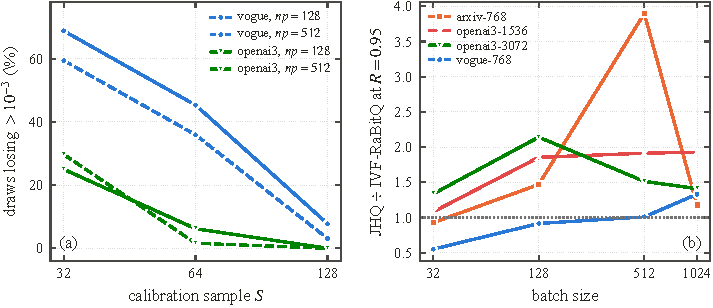
\includegraphics[width=\linewidth]{figs/fig_knobs.pdf}
  \caption{Sensitivity to the two knobs the evaluation varies. (a) The share of
  64 random calibration samples that give up more than $10^{-3}$ of held-out
  recall, against the sample size $S$; solid is $\mathit{nprobe}{=}128$, dashed
  $512$. (b) JHQ over IVF-RaBitQ at matched Recall@10 of $0.95$, against batch
  size, on the four datasets IVF-RaBitQ builds on; above 1 is JHQ ahead.}
  \label{fig:knobs}
\end{figure}

\subsection{RQ5: does batch size change the ordering?}
\label{sec:rq5}
Figure~\ref{fig:knobs}(b) gives matched-recall ratios against IVF-RaBitQ at four
batch sizes, on the four datasets where IVF-RaBitQ builds. It does: JHQ leads at
every measured batch on three of them, while on vogue-768 it crosses parity
between 128 and 512. The frontier ratios of Section~\ref{sec:rq1} are therefore
the batch-1{,}024 point of this sweep and not batch-independent summaries.

\subsection{RQ6: what does the port buy over CPU JHQ?}
\label{sec:rq6cpu}
Figure~\ref{fig:cpu}(a) puts both sides' $(\alpha,\mathit{nprobe})$ envelopes on
one recall axis. Across the four datasets the CPU baseline covers, the GPU
reaches $52$ to $108\times$ the CPU envelope; pinning $\alpha{=}100$ on
\emph{both} sides gives $41$ to $114\times$. We give both because they move in
opposite directions: freedom over $\alpha$ and threads is worth more to the CPU
on some datasets than on others. bge-m3 and stella-trec24 have no CPU
measurement.

Panel~(b) says why the port changes the design and not just the speed: the same
$\alpha$ knob is worth $2.5$ to $3.0\times$ more on the GPU than on the CPU, at
every probe depth. On the CPU the scan dominates and the budget barely matters;
on the GPU the scan is fast enough that refinement becomes the term worth
choosing --- which is what Section~\ref{sec:rq2}'s rule exists to choose.

Two limits. CPU rows below $\mathit{nprobe}{=}128$ are dropped, because 1{,}000
queries finish fast enough there that thread start-up dominates the timer. And
every cell but one is measured once, so these are order-of-magnitude figures:
five repeats on the noisiest cell moved the top vogue ratio from $90\times$ to
$85$.

\begin{figure}[tbp]
  \centering
  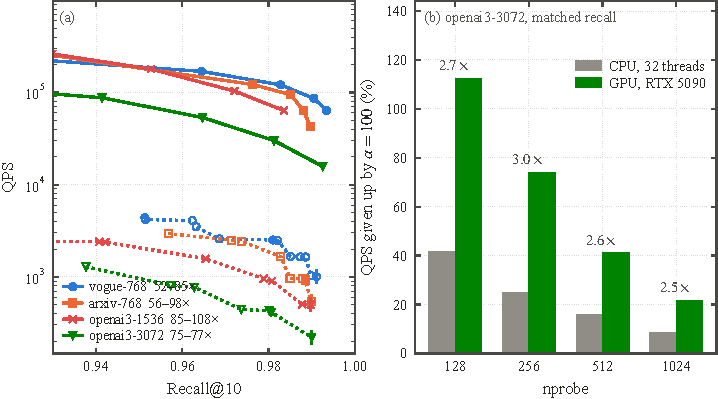
\includegraphics[width=\linewidth]{figs/fig_cpu.pdf}
  \caption{GPU against CPU JHQ at the same index parameters, on the four
  datasets the CPU reference covers. (a) Both sides'
  $(\alpha,\mathit{nprobe})$ envelopes: solid is the GPU, dotted with open
  markers the CPU points the envelope is taken over, and the legend gives each
  dataset's range of matched-recall ratios. (b) What the $\alpha$ budget is
  worth on each processor, at matched recall on openai3-3072 --- the reason the
  budget is worth choosing on a GPU and not on a CPU.}
  \label{fig:cpu}
\end{figure}

\subsection{Construction and memory}
\label{sec:rq6}
Figure~\ref{fig:build} gives cold build times on every dataset. JHQ is the
cheapest to build on all six and the gap widens with $N$: at stella-trec24 it is
$13.4$\,s against $74.3$\,s for CAGRA int8. Accounting must respect caching:
training can be cached while add is not, so taking maxima independently
fabricates a time that never occurred.

Figure~\ref{fig:memory} accounts for what is resident. On the four datasets with
measured VRAM JHQ uses $22$--$40\%$ more than IVF-RaBitQ, and its budget is not
smaller than int8's. The residual level is where it goes --- at stella-trec24
the residual codes alone are most of a 20\,GiB index --- and it is the same
level that buys the high-recall end of Section~\ref{sec:rq1}. JHQ occupies a
different memory--accuracy--throughput point, and still indexes the two largest
datasets where the compared paths fail. The accounting carries an unattributed
component, plotted as such rather than relabelled as allocator overhead.

\begin{figure}[tbp]
  \centering
  
\includegraphics[width=\linewidth]{figs/fig_memory.pdf}
  \caption{Where the resident index sits, by component. (a) Absolute, with the
  measured totals for JHQ and IVF-RaBitQ marked; (b) the same as shares. The
  hatched band is measured total minus the components we can attribute, and is
  shown rather than folded into one of them.}
  \label{fig:memory}
\end{figure}
